%fich.tex
%%%%%%%%%%%%%%%%%%%%%%%%%%%%%%%%%%%%%%%%%%%%%%%%%%%%%%%%%%%%%%%%%%%%%%%%
% Fco. Javier Bóhorquez Ogalla
% Descripción del documento:
	
%%%%%%%%%%%%%%%%%%%%%%%%%%%%%%%%%%%%%%%%%%%%%%%%%%%%%%%%%%%%%%%%%%%%%%%%


%%%%%%%%%%%%%%%%%%%%%%%%%%%%%%%%%%%%%%%%%%%%%%%%%%%%%%%%%%%%%%%%%%%%%%%%
%Clase de documento
\documentclass[12pt, spanish]{article}
%%%%%%%%%%%%%%%%%%%%%%%%%%%%%%%%%%%%%%%%%%%%%%%%%%%%%%%%%%%%%%%%%%%%%%%%


%%%%%%%%%%%%%%%%%%%%%%%%%%%%%%%%%%%%%%%%%%%%%%%%%%%%%%%%%%%%%%%%%%%%%%%%	
%Paquetes de lenguaje:
%%%%%%%%%%%%%%%%%%%%%%%%%%%%%%%%%%%%%%%%%%%%%%%%%%%%%%%%%%%%%%%%%%%%%%%%
\usepackage[utf8]{inputenc}
\usepackage[spanish]{babel}
%\usepackage[spanish, activeacute] {babel}	
%\usepackage[spanish]{babel} 				
%\usepackage[latin1]{inputenc}
%%%%%%%%%%%%%%%%%%%%%%%%%%%%%%%%%%%%%%%%%%%%%%%%%%%%%%%%%%%%%%%%%%%%%%%%

%%%%%%%%%%%%%%%%%%%%%%%%%%%%%%%%%%%%%%%%%%%%%%%%%%%%%%%%%%%%%%%%%%%%%%%%
%Gramatic

\usepackage{/usr/share/texlive/texmf-dist/tex/latex/base/bnf}
%%%%%%%%%%%%%%%%%%%%%%%%%%%%%%%%%%%%%%%%%%%%%%%%%%%%%%%%%%%%%%%%%%%%%%%%

%%%%%%%%%%%%%%%%%%%%%%%%%%%%%%%%%%%%%%%%%%%%%%%%%%%%%%%%%%%%%%%%%%%%%%%%
%Paquetes para encabezados y pie de páginas
%%%%%%%%%%%%%%%%%%%%%%%%%%%%%%%%%%%%%%%%%%%%%%%%%%%%%%%%%%%%%%%%%%%%%%%%
\usepackage{fancyhdr}
%%%%%%%%%
% \pagestyle{fancy} %Si se cambia el estilo de página, antes de empezar 
	%el documento. Esto hace que el emcabezado y pie de página se 
	%quede separado del texto por una línea
%%%%%%%%%	
% \fancyhead{} % Límpia el texto que se está usando como encabezado
%%%%%%%%%
% \fancyhead[OPCIONES]{Encabezado}
	% OPCIONES:
		% L texto a la izquierda
		% C texto centrado
		% R texto a la derecha
		% E página par
		% O pagina impar
	%Ejemplo: 
		% fancyhead [LE] {"Doc. Latex"} 
			% Establece como emcabezado de las páginas pares "Doc Latex"
			% con alineacion a la izquierda
%%%%%%%%%			
% \fancyfoot[OPCIONES]{Píe de pag.}
	% OPCIONES:
		% L C R E O
	%Ejemplo
		% \fancyfoot[LE,RO]{\thepage} 
			% Establece como píe de pág. el número de página. con 
			% alineación a la izq en paginas pares y a la derecha en
			% las impares
%%%%%%%%%			
% \renewcommand{\headrulewidth}{0.4pt}
% \renewcommand{\footrulewidth}{0.4pt}
	% Fija el grosor de la la linea que separa el emcabezado y pie de pág
%%%%%%%%%
% Otros comandos:
%\lhead{}
%\chead{}
%\rhead{}
%\lfoot{}
%\cfoot{}
%%%%%%%%%%%%%%%%%%%%%%%%%%%%%%%%%%%%%%%%%%%%%%%%%%%%%%%%%%%%%%%%%%%%%%%%


%%%%%%%%%%%%%%%%%%%%%%%%%%%%%%%%%%%%%%%%%%%%%%%%%%%%%%%%%%%%%%%%%%%%%%%%
% Paquetes para tamaños y distancias
%%%%%%%%%%%%%%%%%%%%%%%%%%%%%%%%%%%%%%%%%%%%%%%%%%%%%%%%%%%%%%%%%%%%%%%%
\usepackage{anysize} 
%%%%%%%%%%%
% \marginsize{3cm}{2cm}{2cm}{2cm}
	% Controla los márgenes {izquierda}{derecha}{arriba}{abajo}. 
%%%%%%%%%%%%%%%%%%%%%%%%%%%%%%%%%%%%%%%%%%%%%%%%%%%%%%%%%%%%%%%%%%%%%%%%


%%%%%%%%%%%%%%%%%%%%%%%%%%%%%%%%%%%%%%%%%%%%%%%%%%%%%%%%%%%%%%%%%%%%%%%%
%Paquetes de carácteres especiales:
%%%%%%%%%%%%%%%%%%%%%%%%%%%%%%%%%%%%%%%%%%%%%%%%%%%%%%%%%%%%%%%%%%%%%%%%
\usepackage{dsfont}	
%Para representar conjuntos matematicos comunes: Z, N, R...
	% mathds{R}, mathds{N},...
%%%%%%%%%%%%%%%%%%%%%%%%%%%%%%%%%%%%%%%%%%%%%%%%%%%%%%%%%%%%%%%%%%%%%%%%

%%%%%%%%%%%%%%%%%%%%%%%%%%%%%%%%%%%%%%%%%%%%%%%%%%%%%%%%%%%%%%%%%%%%%%%%
%Paquetes para insertar gráficos
%%%%%%%%%%%%%%%%%%%%%%%%%%%%%%%%%%%%%%%%%%%%%%%%%%%%%%%%%%%%%%%%%%%%%%%%
\usepackage[dvips]{graphicx}
\DeclareGraphicsExtensions{.pdf,.png,.jpg} %solo para PDFLaTeX
%%%%%%%%%%%%%%%%%%%%%%%%%%%%%%%%%%%%%%%%%%%%%%%%%%%%%%%%%%%%%%%%%%%%%%%%

%%%%%%%%%%%%%%%%%%%%%%%%%%%%%%%%%%%%%%%%%%%%%%%%%%%%%%%%%%%%%%%%%%%%%%%%
%Paquetes de color:
%%%%%%%%%%%%%%%%%%%%%%%%%%%%%%%%%%%%%%%%%%%%%%%%%%%%%%%%%%%%%%%%%%%%%%%%
\usepackage{color}
%%%%%%%%%%%%%%%%%%%%%%%%%%%%%%%%%%%%%%%%%%%%%%%%%%%%%%%%%%%%%%%%%%%%%%%%
%Definición de colores:
\definecolor{gray97}{gray}{.97}
\definecolor{gray75}{gray}{.75}
\definecolor{gray45}{gray}{.45}
%%%%%%%%%%%%%%%%%%%%%%%%%%%%%%%%%%%%%%%%%%%%%%%%%%%%%%%%%%%%%%%%%%%%%%%%
\usepackage{multicol}

%%%%%%%%%%%%%%%%%%%%%%%%%%%%%%%%%%%%%%%%%%%%%%%%%%%%%%%%%%%%%%%%%%%%%%%%
%Paquete de listado de código:
%%%%%%%%%%%%%%%%%%%%%%%%%%%%%%%%%%%%%%%%%%%%%%%%%%%%%%%%%%%%%%%%%%%%%%%%
\usepackage{listings}
%%%%%%%%%%%%%%%%%%%%%%%%%%%%%%%%%%%%%%%%%%%%%%%%%%%%%%%%%%%%%%%%%%%%%%%%
%Configuración del listado:

\lstset { 
	frame=Ltb,
     framerule=0pt,
     aboveskip=0.2cm,
     framextopmargin=0.3pt,
     framexbottommargin=0.2pt,
     framexleftmargin=0.3cm,
     framesep=0pt,
     rulesep=.1pt,
     tabsize=2,
     backgroundcolor=\color{gray97},
     rulesepcolor=\color{black},
     %
     stringstyle=\ttfamily,
     showstringspaces = false,
     basicstyle=\scriptsize\ttfamily,
     commentstyle=\color{gray45},
     keywordstyle=\bfseries,
   	%
     numbers=left,
     numbersep=1pt,
     numberstyle=\tiny,
     numberfirstline = false,
     breaklines=true,
}
%%%%%%%%%%%%%%%%%%%%%%%%%%%%%%%%%%%%%%%%%%%%%%%%%%%%%%%%%%%%%%%%%%%%%%%%


%%%%%%%%%%%%%%%%%%%%%%%%%%%%%%%%%%%%%%%%%%%%%%%%%%%%%%%%%%%%%%%%%%%%%%%%
%Indexado. Índice alfabeticos
\usepackage{makeidx}
\makeindex %para habilitar indices
%%%%%%%%%%%%%%%%%%%%%%%%%%%%%%%%%%%%%%%%%%%%%%%%%%%%%%%%%%%%%%%%%%%%%%%%
%Forma de uso:
% \index{clave} %Para crear un indice de materia
% Supongase que queremos meter en el indice alfabetico referencias a 
% las paginas donde se hace referencia a la clave Producto escalar
% en tal caso en cada una de las páginas pondremos \index{Producto escalar}
% \printindex %Para imprimir el índice alfabetico

% Es necesario una doble compilación del documento. La primera genera un 
% fichero.idx el cual tendremos que procesar con la aplicación makeindex
%tras procesarlo se creará un fichero.ind que contendra el código Latex 
% que se inserta en el documento original. 
% Tras la segunda compilación del documento original se sustituira el
% comando \printindex por el contenido del fichero.ind 

%Podemos cambiar el formato de la clave:
%Ejemplo     				&    	Entrada 		&	Comentario
%\index{hola}				&         hola, 1   	&	Entrada simple
%\index{hola!Pedro}			&		 Pedro, 3 	&	Subentrada bajo ‘hola’
%\index{Juan@\textsl{Juan}}  	&		Juan, 2    	&	Entrada con diseño                        
%\index{Pepa@\textbf{Pepa}}	&		Pepa, 7    	&	Igual que antes
%\index{Loli|textbf}		&		Loli, 3    	&	No de página con diseño                     
%\index{Soraya|textit}		&		Soraya, 5  	&	Igual que antes
%%%%%%%%%%%%%%%%%%%%%%%%%%%%%%%%%%%%%%%%%%%%%%%%%%%%%%%%%%%%%%%%%%%%%%%%


%%%%%%%%%%%%%%%%%%%%%%%%%%%%%%%%%%%%%%%%%%%%%%%%%%%%%%%%%%%%%%%%%%%%%%%%


%%%%%%%%%%%%%%%%%%%%%%%%%%%%%%%%%%%%%%%%%%%%%%%%%%%%%%%%%%%%%%%%%%%%%%%%
%Estilo de página
%%%%%%%%%%%%%%%%%%%%%%%%%%%%%%%%%%%%%%%%%%%%%%%%%%%%%%%%%%%%%%%%%%%%%%%%
%\textwidth 6.75in								  %ancho de texto
%\oddsidemargin -0.2in							%margen izquierdo 
\parskip 0.2in									%espacio parrafos
%%%%%%%%%%%%%%%%%%%%%%%%%%%%%%%%%%%%%%%%%%%%%%%%%%%%%%%%%%%%%%%%%%%%%%%%
\newenvironment{changemargin}[2]{%
\begin{list}{}{%
\setlength{\topsep}{300pt}%
\setlength{\leftmargin}{#1}%
\setlength{\rightmargin}{#2}%
\setlength{\listparindent}{\parindent}%
\setlength{\itemindent}{\parindent}%
\setlength{\parsep}{\parskip}%
}%
\item[]}{\end{list}}
%%%%%%%%%%%%%%%%%%%%%%%%%%%%%%%%%%%%%%%%%%%%%%%%%%%%%%%%%%%%%%%%%%%%%%%%
\usepackage{float}
\restylefloat{table}
\usepackage{placeins}
\usepackage{framed}
\usepackage{epsf}
%%%%%%%%%%%%%%%%%%%%%%%%%%%%%%%%%%%%%%%%%%%%%%%%%%%%%%%%%%%%%%%%%%%%%%%%

\usepackage{titlesec}

\setcounter{secnumdepth}{4}

\titleformat{\paragraph}
{\normalfont\normalsize\bfseries}{\theparagraph}{1em}{}
\titlespacing*{\paragraph}
{0pt}{3.25ex plus 1ex minus .2ex}{1.5ex plus .2ex}


%%%%%%%%%%%%%%%%%%%%%%%%%%%%%%%%%%%%%%%%%%%%%%%%%%%%%%%%%%%%%%%%%%%%%%%%	
%datos del documento
\author{Gramática \\\\\ Fco. Javier Bohórquez Ogalla}						%autor
\date{}														%fecha

\title{ 
\begin{center}

\includegraphics[scale=0.5]{logo-doc.png}
\end{center} 
}
%%%%%%%%%%%%%%%%%%%%%%%%%%%%%%%%%%%%%%%%%%%%%%%%%%%%%%%%%%%%%%%%%%%%%%%%

%%%%%%%%%%%%%%%%%%%%%%%%%%%%%%%%%%%%%%%%%%%%%%%%%%%%%%%%%%%%%%%%%%%%%%%%
%Documento:
%%%%%%%%%%%%%%%%%%%%%%%%%%%%%%%%%%%%%%%%%%%%%%%%%%%%%%%%%%%%%%%%%%%%%%%%
\lstdefinestyle{nonumbers}{numbers=none}
\begin{document}

\maketitle
\pagebreak
\tableofcontents
\pagebreak
\section{Vista general}
En esta sección se presenta la gramática del lenguaje, para ello 
se procede a una descripción de las reglas gramaticales
 mediante el lenguaje EBNF (Extended Backus–Naur Form) 
usado para expresar gramáticas libres de contexto. Además cada regla se acompaña de un
diagrama sintáctico o diagrama de carril. 

Una gramática $G$ se define formalmente como sigue:

$$G = (V_t,V_n, P, S)$$

De forma que:

\begin{description}
\item[$V_t$] es un conjunto finito de símbolos no terminales
\item[$V_n$] es un conjunto finito de símbolos terminales
\item[$P$] es un conjunto finito de reglas de producción
\item[$S\ \epsilon\ V_n$] es el símbolo inicial
\end{description}

Las reglas de producción de una grmática libre de contexto tiene la forma siguiente forma:

$$V_n\ \rightarrow\ (V_t\ \cup\ V_n)^*$$ 

La gramática libre de contexto abordada tiene como símbolo inicial 
el no terminal $program$. Se comienza pues describiendo las reglas de producción 
relicionadas con este símbolo, siguiendo con las reglas de producción derivadas 
de esta. 

Las reglas de producción se organizan en niveles como sigue:

\begin{center}
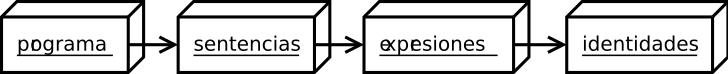
\includegraphics[scale=0.7]{diagram/omi.png} \\
\end{center}

Estos niveles son dados a partir del nivel de abstracción del significado 
semántico que encierran las reglas de producción contenidas en los mismos.

Las reglas de producción correspondientes al nivel de programa 
son las más genéricas y se valen de las de la siguiente nivel para 
su definición. Estas definen el programa como una secuencia de
sentencias. La gramática descrita contempla el programa vacío, es decir,
el programa que no contiene ninguna sentencia.

Las reglas de producción del nivel de sentencia se definen a 
partir de expresiones o de otras sentencias. Una sentencia contiene un significado semántico
operativo de valor para el programa. Cabe decir que una expresión por si sola 
puede constituir una sentencia. La gramática expuesta describe la sentencia
vacía, esta es una sentencia que no tienen ningún significado semántico.

Las expresiones son la unidad mínima con significado semántico atribuido por 
el lenguaje. La mayoría de expresiones se definen a partir de identidades, 
sin embargo algunos tipos de expresiones, como las funciones, pueden formarse
a partir de reglas de más alto nivel de abstracción semantica. Por otro lado las 
reglas de producción correspondiente a las expresiones están organizadas en niveles según
la prioridad atribuida en su resolución.

Las identidades son reglas de producción atómicas, componiéndose únicamente de símblos no terminales. 
Tienen un significado semántico asociado de forma directa. Normalmente este valor viene dado por 
el análisis léxico.  
 
% ----------------------------------------------------------------------
\section{Programa}
\begin{multicols}{2}
\begin{lstlisting}[style=nonumbers]
program  ::=  stmts
            | empty
\end{lstlisting}  
\columnbreak
\begin{center}
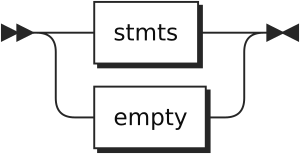
\includegraphics[scale=0.7]{diagram/program.png} \\
\end{center}
\end{multicols}
% ----------------------------------------------------------------------
\section{Sentencias}
\subsection{Secuecia de sentencias}
\begin{multicols}{2}
\begin{lstlisting}[style=nonumbers]
stmts    ::=   stmt ";" stmts
            |  stmt ";"?
            |  stmtb 
            |  label stmts
            |  ";"
\end{lstlisting}  	
\columnbreak
\begin{center}
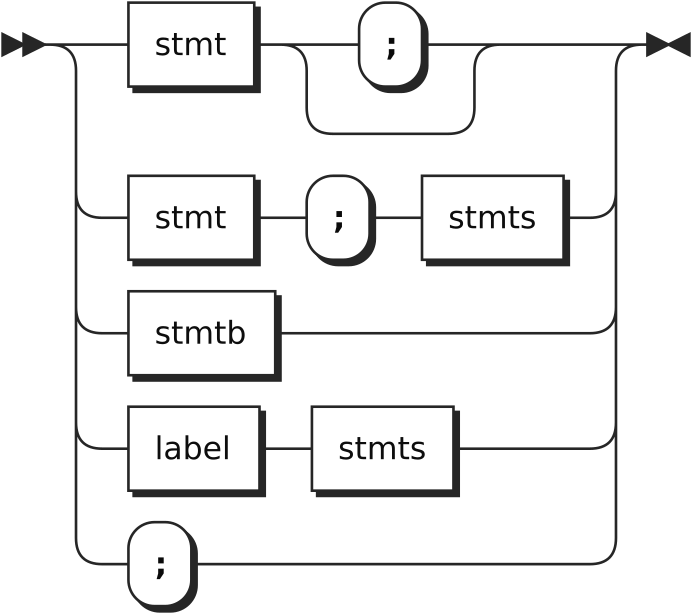
\includegraphics[scale=0.7]{diagram/stmts.png} \\
\end{center}
\end{multicols}
\pagebreak
\subsection{Sentencia de bloque}
\begin{multicols}{2}
\begin{lstlisting}[style=nonumbers]
stmtb ::=   if
         |  while
         |  dowhile
         |  for
         |  foreach
         |  break
         |  switch
         |  iloop
         |  trycatch
         |  class
         |  with
\end{lstlisting}  	
\columnbreak
\begin{center}
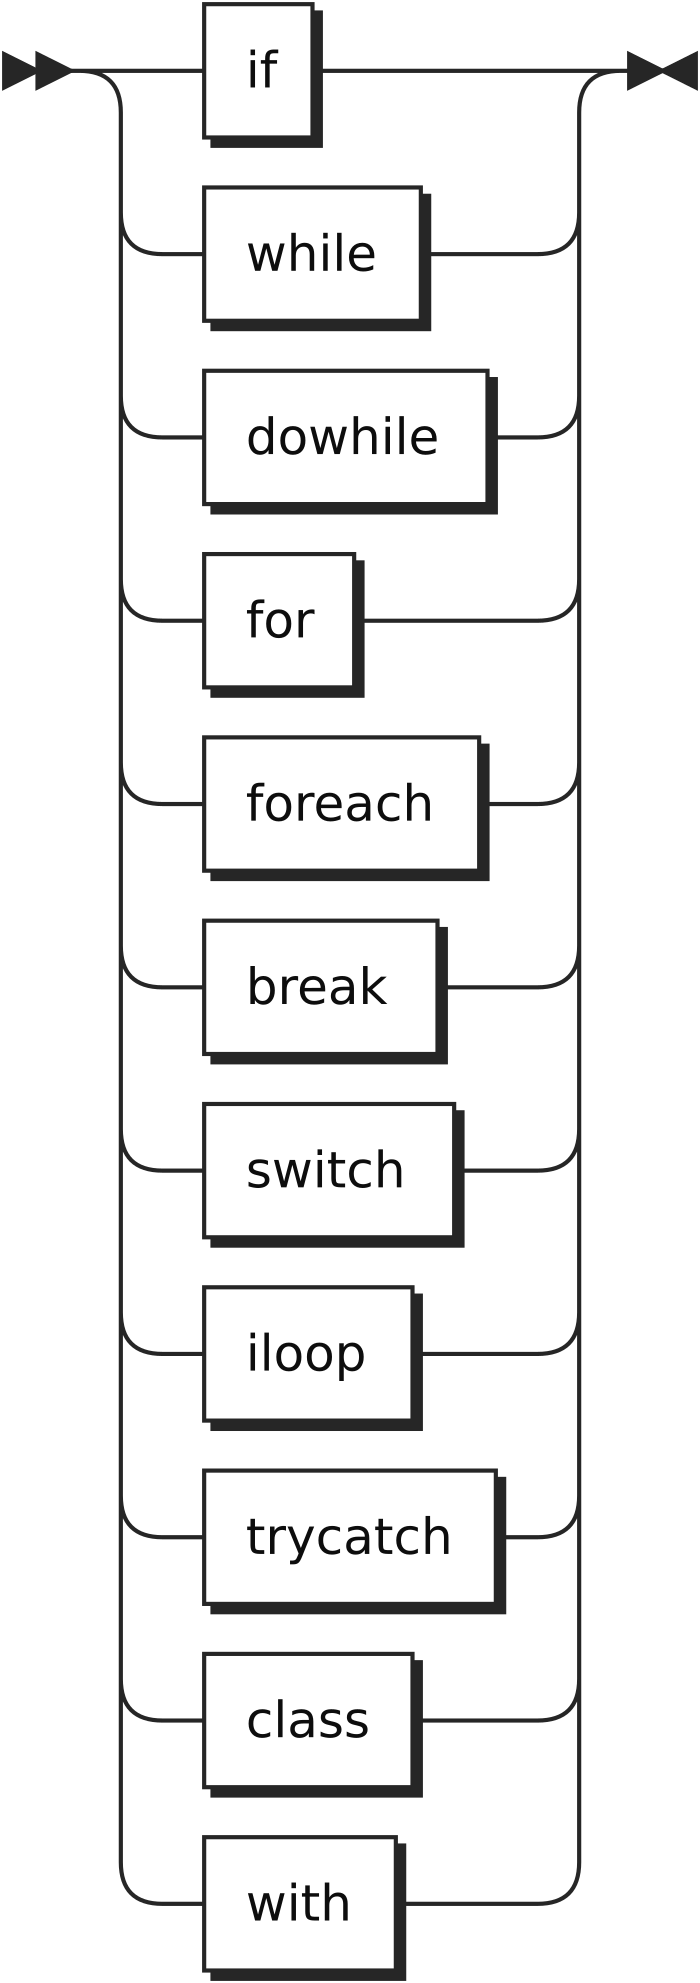
\includegraphics[scale=0.7]{diagram/stmtb.png} \\
\end{center}
\end{multicols}
\subsubsection{Sentencia de control: if}
\begin{lstlisting}[style=nonumbers,
    basicstyle=\tiny, %or \small or \footnotesize etc.
]
if ::= "if" exp ("{" stmts? "}" | stmt ";" | stmtb) elif* ("else" ("{" stmts? "}" | stmt ";" | stmtb))?

elif ::=  "elif" exp ( "{" stmts? "}" | stmt ";" | stmtb ) 
\end{lstlisting}  	
\begin{center}
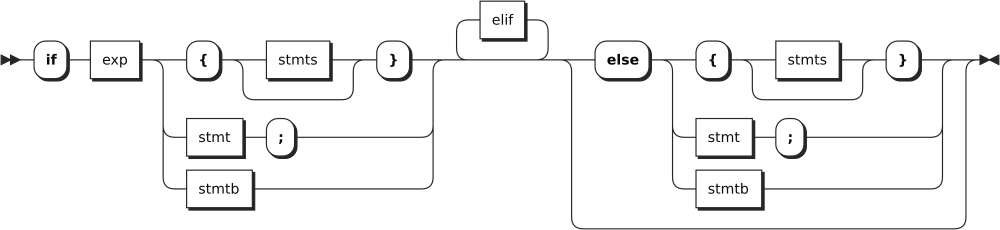
\includegraphics[scale=0.5]{diagram/if.png} \\
\end{center}
\begin{center}
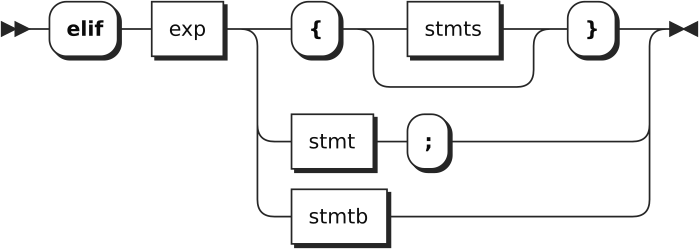
\includegraphics[scale=0.5]{diagram/elif.png} \\
\end{center}

\subsubsection{Sentencia de control: while}
\begin{multicols}{2}
\begin{lstlisting}[style=nonumbers,
    basicstyle=\tiny]
while ::= 
   "while" exp ("{" stmts? "}" | stmt ";" | stmtb)
\end{lstlisting}  	
\columnbreak
\begin{center}
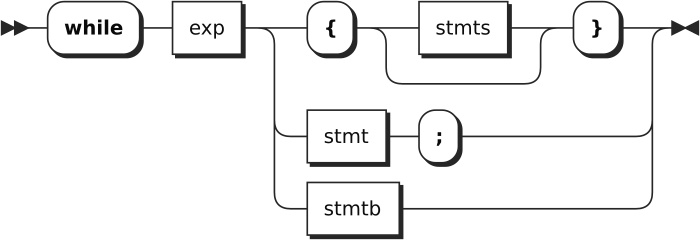
\includegraphics[scale=0.5]{diagram/while.png} \\
\end{center}
\end{multicols}

\subsubsection{Sentencia de control: do...while}
\begin{lstlisting}[style=nonumbers]
dowhile ::=  "do" ( "{" stmts? "}" | stmt ";" | stmtb ) "while" exp ";"
\end{lstlisting}  	
\begin{center}
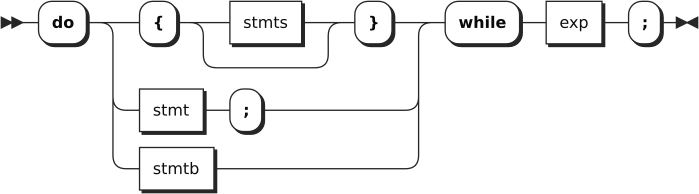
\includegraphics[scale=0.5]{diagram/dowhile.png} \\
\end{center}

\subsubsection{Sentencia de control: for}
\begin{lstlisting}[style=nonumbers]
for ::= "for" "("? exp? ";" exp? ";" exp? ")"? ( "{" stmts? "}" | stmt ";" | stmtb )
\end{lstlisting}  	
\begin{center}
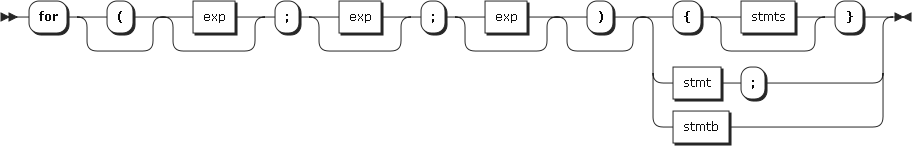
\includegraphics[scale=0.4]{diagram/for.png} \\
\end{center}
\subsubsection{Sentencia de control: forearch}
\begin{lstlisting}[style=nonumbers,basicstyle=\tiny]
foreach ::= 
   "for" "("?(id (":" id)? "in" exp | exp "as" id (":" id)?)")"? ("{" stmts? "}" | stmt ";" | stmtb)
\end{lstlisting}  	
\begin{center}
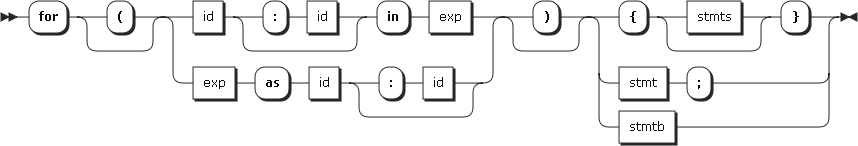
\includegraphics[scale=0.4]{diagram/foreach.png} \\
\end{center}
\pagebreak
\subsubsection{Sentencia de control: switch}
\begin{lstlisting}[style=nonumbers]
switch ::= "switch" "(" exp ")" "{" cases? "}"

cases ::= "case" exp ":" ( stmts cases | stmts | cases )
   |  "default" ":" stmts
\end{lstlisting}  	
\begin{center}
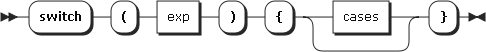
\includegraphics[scale=0.4]{diagram/switch.png} \\
\end{center}
\begin{center}
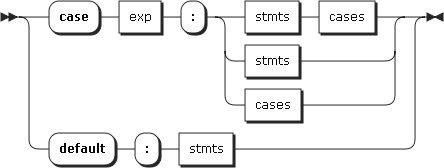
\includegraphics[scale=0.4]{diagram/cases.png} \\
\end{center}

\subsubsection{Sentencia de control: iloop}
\begin{lstlisting}[style=nonumbers,basicstyle=\tiny]
iloop ::= "$" "(" exp ( "as" id (":" id)? )? ("," exp )? ")" ( "{" stmts? "}" | stmt ";" | stmtb )

iloop_access ::=  "$"
               |  "$" "{" NUM "}"
\end{lstlisting}  	
\begin{center}
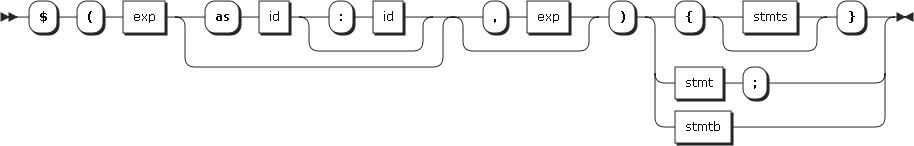
\includegraphics[scale=0.4]{diagram/iloop.png} \\
\end{center}
\begin{center}
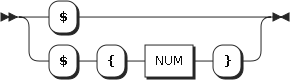
\includegraphics[scale=0.4]{diagram/iloop_access.png} \\
\end{center}

\subsubsection{Sentencia de control: try...catch}

\begin{lstlisting}[style=nonumbers,basicstyle=\tiny]
trycatch ::= 
 "try" ( "{" stmts? "}" | stmt ";" | stmtb ) catch "(" id ")" ( "{" stmts? "}" | stmt ";" |  stmtb )
\end{lstlisting}  	
\begin{center}
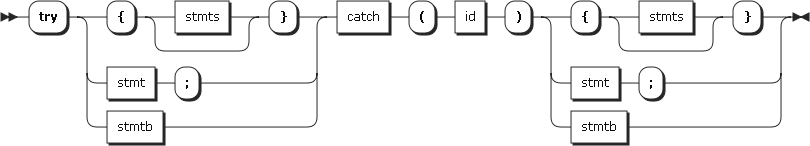
\includegraphics[scale=0.4]{diagram/trycatch.png} \\
\end{center}

\pagebreak
\subsubsection{Sentencia de control: with}
\begin{multicols}{2}
\begin{lstlisting}[style=nonumbers,basicstyle=\tiny]
with ::= 
 "with" exp ( "{" stmts? "}" | stmt ";" | stmtb )
\end{lstlisting}  	
\columnbreak
\begin{center}
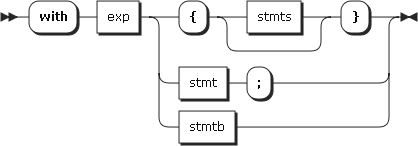
\includegraphics[scale=0.4]{diagram/with.png} \\
\end{center}
\end{multicols}


\subsection{Sentencia simple}
\begin{multicols}{2}
\begin{lstlisting}[style=nonumbers]
stmt  ::=   exp
         |  "<<" exp
         |  ">>" ("[" exp "]")? id
         |  "goto" exp
         |  "include" exp
         |  "return" exp?
         |  "sleep" exp 
         |  "load" exp 
         |  "typeof" id 
         |  "datinfo" exp
         |  "exit"
         |  "throw" exp
         |  "global" identity
         |  "break" num? ";"
         |  "continue" num? ";"
\end{lstlisting}  	
\columnbreak
\begin{center}
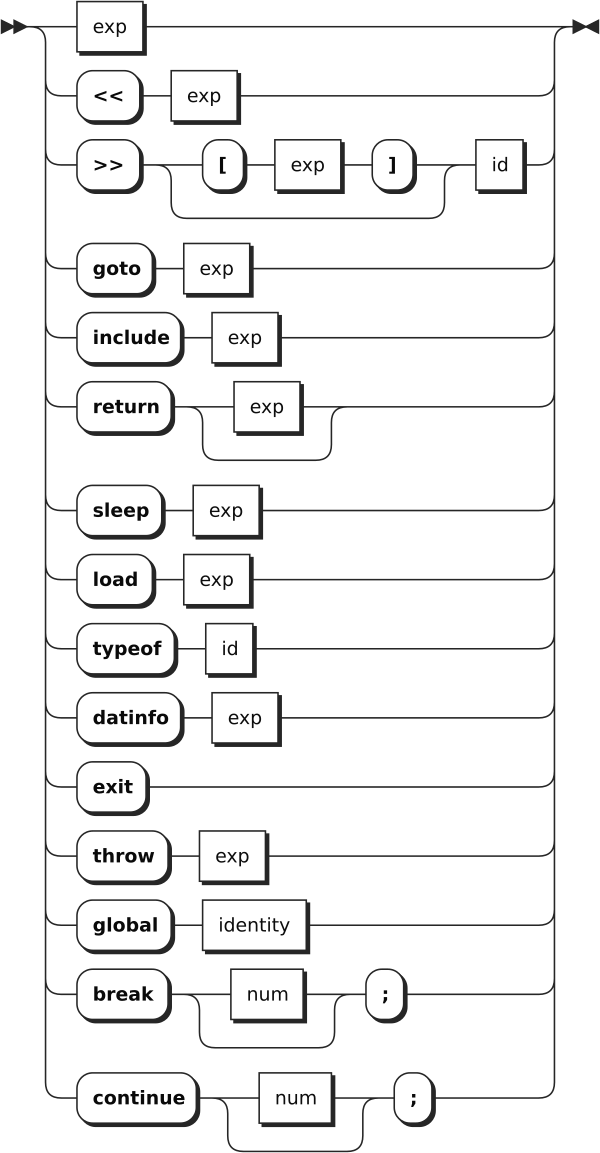
\includegraphics[scale=0.6]{diagram/stmt.png} \\
\end{center}
\end{multicols}

\subsection{Etiquetas}
\begin{multicols}{2}
\begin{lstlisting}[style=nonumbers]
label ::=   id ":"
\end{lstlisting}  	
\columnbreak
\begin{center}
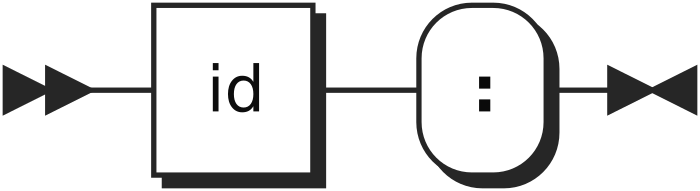
\includegraphics[scale=0.7]{diagram/label.png} \\
\end{center}
\end{multicols}
\pagebreak
\subsection{Nombres de espacios}
\begin{multicols}{2}
\begin{lstlisting}[style=nonumbers, basicstyle=\tiny]      
namespace ::=  namespace "::" id
            |  id "::" id
            |  "parent" "::" id
            |  "static" "::" id
\end{lstlisting}  
\columnbreak	
\begin{center}
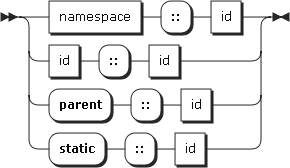
\includegraphics[scale=0.4]{diagram/namespace.png} \\
\end{center}
\end{multicols}
\subsection{Clases}
\begin{lstlisting}[style=nonumbers]
class ::= "class" id ("extends" id )? "{" class_stmts? "}"
\end{lstlisting}  	
\begin{center}
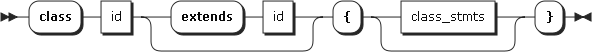
\includegraphics[scale=0.6]{diagram/class.png} \\
\end{center}
\subsubsection{Métodos y atributos}
\begin{lstlisting}[style=nonumbers]
class_stmts ::= 
   (("static"|"private"|"private" "static"|"static" "private")? (function|id|assig))*

\end{lstlisting}  	
\begin{center}
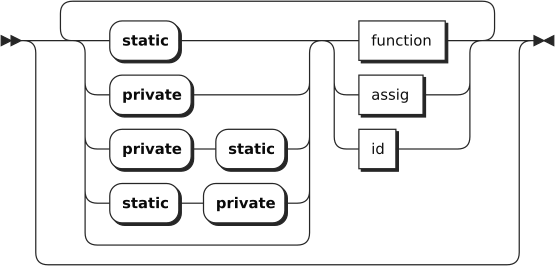
\includegraphics[scale=0.7]{diagram/class_stmts.png} \\
\end{center}
% ----------------------------------------------------------------------
% ----------------------------------------------------------------------
\section {Expresiones}
\begin{multicols}{2}
\begin{lstlisting}[style=nonumbers]      
exp ::= op1
\end{lstlisting}  
\columnbreak	
\begin{center}

\includegraphics[scale=0.5]{diagram/exp.png} \\
\end{center}
\end{multicols}
\subsection{Operadores lógicos}
\subsubsection{Or lógico}
\begin{multicols}{2}
\begin{lstlisting}[style=nonumbers]      
op1 ::=  op1 ( "||" | "or" ) op2
      |  op2
\end{lstlisting}  
\columnbreak	
\begin{center}
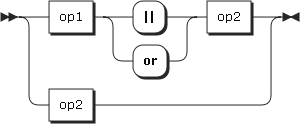
\includegraphics[scale=0.6]{diagram/lop1.png} \\
\end{center}
\end{multicols}

\subsubsection{And lógico}
\begin{multicols}{2}
\begin{lstlisting}[style=nonumbers]      
op2 ::=  op2 ( "&&" | "and" ) op3
      |  op3
\end{lstlisting}  
\columnbreak	
\begin{center}
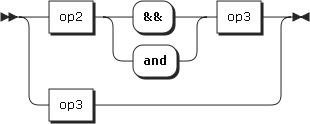
\includegraphics[scale=0.6]{diagram/op2.png} \\
\end{center}
\end{multicols}

\subsubsection{Negación lógica}
\begin{multicols}{2}
\begin{lstlisting}[style=nonumbers]      
op3 ::=  "!" op3 
      |  op4
\end{lstlisting}  
\columnbreak	
\begin{center}
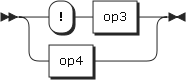
\includegraphics[scale=0.6]{diagram/op3.png} \\
\end{center}
\end{multicols}

\subsubsection{Comparaciones}
\begin{multicols}{2}
\begin{lstlisting}[style=nonumbers]      
op4 ::=  op4 "<" op5
      |  op4 "<=" op5
      |  op4 ">" op5
      |  op4 ">=" op5
      |  op4 "==" op5
      |  op4 "!=" op5
      |  op4 "===" op5
      |  op4 "!==" op5
      |  op5
\end{lstlisting}  
\columnbreak	
\begin{center}
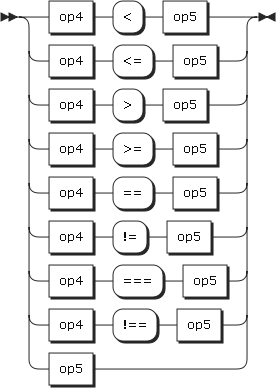
\includegraphics[scale=0.5]{diagram/op4.png} \\
\end{center}
\end{multicols}

\subsection{Operadores aritméticos}
\subsubsection{Suma y diferencia}
\begin{multicols}{2}
\begin{lstlisting}[style=nonumbers]      
op5 ::= op5 "+" op6
      |  op5  "-" op6
      |  op6
\end{lstlisting}  
\columnbreak	
\begin{center}
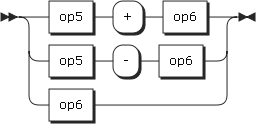
\includegraphics[scale=0.5]{diagram/op5.png} \\
\end{center}
\end{multicols}

\subsubsection{Producto y división}
\begin{multicols}{2}
\begin{lstlisting}[style=nonumbers]      
op6  ::= op6 "*" op7
      |  op6 "/" op7
      |  op7
\end{lstlisting}  
\columnbreak	
\begin{center}
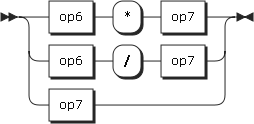
\includegraphics[scale=0.5]{diagram/op6.png} \\
\end{center}
\end{multicols}

\subsubsection{Potencia y módulo}
\begin{multicols}{2}
\begin{lstlisting}[style=nonumbers]      
op7  ::= op7 "^" op8
      |  op7 "%" op8
      |  op8
\end{lstlisting}  
\columnbreak	
\begin{center}
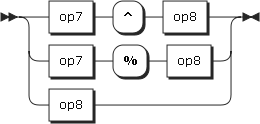
\includegraphics[scale=0.5]{diagram/op7.png} \\
\end{center}
\end{multicols}

\subsection{Operadores cadenas de caracteres}
\subsubsection{Concatenación}
\begin{multicols}{2}
\begin{lstlisting}[style=nonumbers]      
op8 ::=  op8 "." op9
      |  op9
\end{lstlisting}  
\columnbreak	
\begin{center}
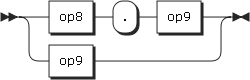
\includegraphics[scale=0.5]{diagram/op8.png} \\
\end{center}
\end{multicols}
\subsubsection{Flujo}
\begin{multicols}{2}
\begin{lstlisting}[style=nonumbers]      
op9  ::= call "<<" op9
      |  call
\end{lstlisting}  
\columnbreak	
\begin{center}
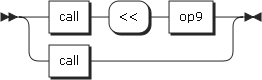
\includegraphics[scale=0.5]{diagram/op9.png} \\
\end{center}
\end{multicols}

\subsection{Llamadas}
\begin{multicols}{2}
\begin{lstlisting}[style=nonumbers]      
call ::= call "(" list? ")"
      |  opc
\end{lstlisting}  
\columnbreak	
\begin{center}
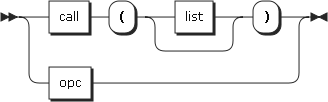
\includegraphics[scale=0.5]{diagram/call.png} \\
\end{center}
\end{multicols}

\subsection{Operadores condicionales}
\begin{multicols}{2}
\begin{lstlisting}[style=nonumbers]      
opc ::=  tern
      |  nullcoalescing
      |  unity
\end{lstlisting}  
\columnbreak	
\begin{center}
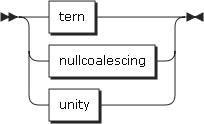
\includegraphics[scale=0.5]{diagram/opc.png} \\
\end{center}
\end{multicols}
\subsubsection{Operador ternario}
\begin{multicols}{2}
\begin{lstlisting}[style=nonumbers]      
tern ::= exp "?" exp? ":" exp
   |  exp "?" exp
\end{lstlisting}  
\columnbreak	
\begin{center}
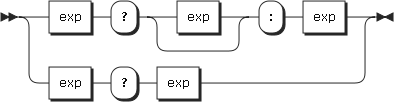
\includegraphics[scale=0.5]{diagram/tern.png} \\
\end{center}
\end{multicols}
\subsubsection{Null coalescing}
\begin{multicols}{2}
\begin{lstlisting}[style=nonumbers]      
nullcoalescing ::= "[[" list "]]"
\end{lstlisting}  
\columnbreak	
\begin{center}

\includegraphics[scale=0.5]{diagram/nullcoalescing.png} \\
\end{center}
\end{multicols}

\pagebreak
\subsection{Operadores unitarios}
\begin{multicols}{2}
\begin{lstlisting}[style=nonumbers]      
unity ::=   inc_dec
         |  assignation_exp
         |  cast
         |  logical_func
         |  arith_func
         |  array_func
         |  string_func
         |  regexp_func
         |  iloop_access
         |  class_exp
         |  func_exp
         |  file
         |  date
         |  process
         |  generator
         |  environments
         |  array
         |  identity
\end{lstlisting}  
\columnbreak	
\begin{center}
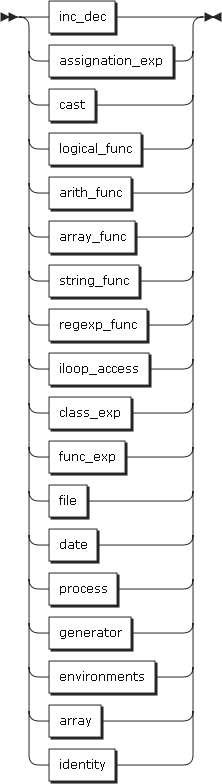
\includegraphics[scale=0.5]{diagram/unity.png} \\
\end{center}
\end{multicols}

\subsubsection{Incrementos y decrementos}
\begin{multicols}{2}
\begin{lstlisting}[style=nonumbers]      
inc_dec ::= "++" exp
         |  exp "++"
         |  "--" exp
         |  exp "--"
\end{lstlisting}  
\columnbreak	
\begin{center}
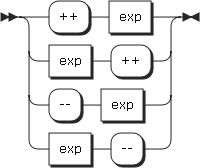
\includegraphics[scale=0.5]{diagram/inc_dec.png} \\
\end{center}
\end{multicols}
\pagebreak
\subsubsection{Conversión de tipos}
\begin{multicols}{2}
\begin{lstlisting}[style=nonumbers]      
cast ::= "int" exp
      |  "float" exp
      |  "bool" exp
      |  "str" exp
\end{lstlisting}  
\columnbreak	
\begin{center}
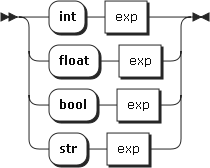
\includegraphics[scale=0.5]{diagram/cast.png} \\
\end{center}
\end{multicols}



\subsubsection{Accesos}
\begin{multicols}{2}
\begin{lstlisting}[style=nonumbers, basicstyle=\tiny]      
access ::=  access "->" id
         |  access "[" exp? "]"
         |  call "->" id
         |  call "[" exp? "]"
\end{lstlisting}  
\columnbreak	
\begin{center}
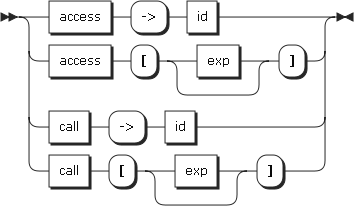
\includegraphics[scale=0.4]{diagram/access.png} \\
\end{center}
\end{multicols}

\subsection{Asignaciones}
\begin{multicols}{2}
\begin{lstlisting}[style=nonumbers, basicstyle=\tiny]      
assignation ::=   
 (id | assignation | access)  "=" "&"? exp
\end{lstlisting}  
\columnbreak	
\begin{center}
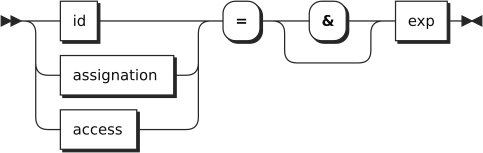
\includegraphics[scale=0.5]{diagram/assignation.png} \\
\end{center}
\end{multicols}
\subsection{Funciones}
\begin{lstlisting}[style=nonumbers]
function ::= "~" id "(" params_val? ")" "{" stmts? "}"
\end{lstlisting}
\begin{center}
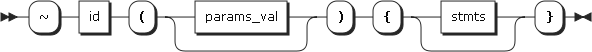
\includegraphics[scale=0.5]{diagram/function.png} \\
\end{center}
\subsubsection {Función lambda}
\begin{lstlisting}[style=nonumbers]
function_lambda ::= "~" "(" params_val? ")" "{" stmts? "}"
    | "~" params_val ":" exp
    | "~&" id
\end{lstlisting}
\begin{center}
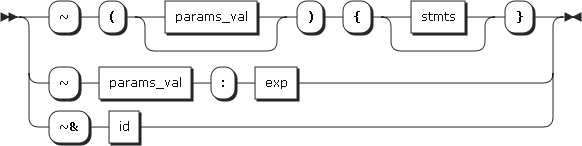
\includegraphics[scale=0.5]{diagram/function_lambda.png} \\
\end{center}
\subsubsection {Cálculo parcial}
\begin{lstlisting}[style=nonumbers]
function_partial ::= "P" "[" params_val "]" "(" id ")"
   |  "P" "[" params_val "]" "(" function_exp ")"
   |  "P" "[" params_val "]" "(" arrayexp ")"
\end{lstlisting}
\begin{center}
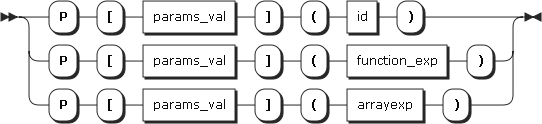
\includegraphics[scale=0.5]{diagram/function_partial.png} \\
\end{center}
\subsubsection {Función de contexto}
\begin{lstlisting}[style=nonumbers]
function_context ::= "~>"
\end{lstlisting}
\begin{center}

\includegraphics[scale=0.5]{diagram/function_context.png} \\
\end{center}


\subsection{Decoradores}
\begin{lstlisting}[style=nonumbers]
decorator ::= "~~" id "(" params_val? ")" "{" stmts? "}"
\end{lstlisting}
\begin{center}
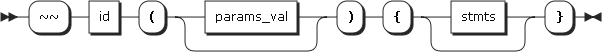
\includegraphics[scale=0.5]{diagram/decorator.png} \\
\end{center}
\subsubsection{Decorador lambda}
\begin{lstlisting}[style=nonumbers]
decorator_lambda ::= "~~" "(" params_val? ")" "{" stmts? "}"
\end{lstlisting}
\begin{center}
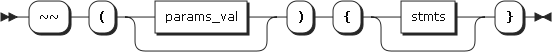
\includegraphics[scale=0.5]{diagram/function_decorator.png} \\
\end{center}




\pagebreak
\subsection{Operadores clases y objetos}
\begin{multicols}{2}
\begin{lstlisting}[style=nonumbers]      
class_exp ::=  "new" id ("(" list? ")")?
            |  "this" 
            |  "parent"
            |  namespace
\end{lstlisting}  
\columnbreak	
\begin{center}
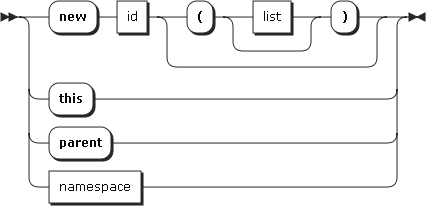
\includegraphics[scale=0.5]{diagram/class_exp.png} \\
\end{center}
\end{multicols}

\subsection{Funciones del lenguaje}
\subsubsection{Funciones lógicas}
\begin{multicols}{2}
\begin{lstlisting}[style=nonumbers]      
logical_func ::=  "isnull" exp
               |  "empty" exp
\end{lstlisting}  
\columnbreak	
\begin{center}
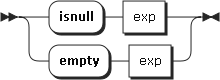
\includegraphics[scale=0.5]{diagram/logical_func.png} \\
\end{center}
\end{multicols}

\subsubsection{Funciones aritméticas}
\begin{multicols}{2}
\begin{lstlisting}[style=nonumbers]      
arith_func ::= "size" exp
            |  "sizeof" exp
\end{lstlisting}  
\columnbreak	
\begin{center}
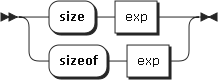
\includegraphics[scale=0.5]{diagram/arith_func.png} \\
\end{center}
\end{multicols}

\subsubsection{Funciones cadenas de caracteres}
\begin{lstlisting}[style=nonumbers]      
string_func ::=   "sprintf" "(" exp "," exp ")"
               |  "str_replace" "(" exp "," exp "," exp ("," exp)? ")"
               |  "str_subreplace" "(" exp "," exp "," exp "," exp ")"
               |  "str_find" "(" exp "," exp ("," exp)? ")"
               |  "str_upper" "(" exp ")"
               |  "str_lower" "(" exp ")"
\end{lstlisting}  
\begin{center}
\includegraphics[scale=0.4]{diagram/string_func.png} \\
\end{center}

\subsubsection{Funciones arrays}
\begin{multicols}{2}
\begin{lstlisting}[style=nonumbers]      
array_func ::= 
 "array_explode" "(" exp "," exp ")"
 |  "array_implode" "(" exp "," exp ")"
 |  "array_chunck" "(" exp "," exp ")"
 |  "array_reduce" "(" exp "," exp ")"
\end{lstlisting}  
\columnbreak	
\begin{center}
\includegraphics[scale=0.5]{diagram/array_func.png} \\
\end{center}
\end{multicols}

\subsubsection{Funciones expresiones regulares}
\begin{lstlisting}[style=nonumbers]      
regexp_func ::=   "regexp" "(" exp ")"
               |  "search" "(" exp "," exp ("," list)? ")"
               |  "match" "(" exp "," exp ")"
\end{lstlisting}  
\begin{center}
\includegraphics[scale=0.5]{diagram/regexp_func.png} \\
\end{center}

\subsubsection{Funciones fechas y tiempo}
\begin{multicols}{2}
\begin{lstlisting}[style=nonumbers]      
date ::= "date" "(" exp ")"
      |  "time" ("(" ")")
\end{lstlisting}  
\columnbreak	
\begin{center}
\includegraphics[scale=0.5]{diagram/date.png} \\
\end{center}
\end{multicols}

\subsubsection{Funciones acceso a entorno}
\begin{multicols}{2}
\begin{lstlisting}[style=nonumbers]      
environment ::= "getenv" "(" exp ")"
\end{lstlisting}  
\columnbreak	
\begin{center}
\includegraphics[scale=0.4]{diagram/environment.png} \\
\end{center}
\end{multicols}

\pagebreak
\subsubsection{Funciones ficheros}
\begin{multicols}{2}
\begin{lstlisting}[style=nonumbers, basicstyle=\tiny]      
file ::= "file" "(" exp ("," exp)? ")"
   |  "fput" "(" exp "," exp ")"
   |  "fwrite" "(" exp "," exp ")"
   |  "fappend" "(" exp "," exp ")"
   |  "fget" "(" exp ("," exp)? ")"
   |  "fread" "(" exp ")"
   |  "fclose" "(" exp ")"
   |  "fseek" "(" exp "," exp ("," fposs)? ")"
   |  "ftell" "(" exp ")"

fpos ::= FSET
      |  FCUR
      |  FEND
\end{lstlisting}  
\begin{center}
\includegraphics[scale=0.4]{diagram/fpos.png} \\
\end{center}
\columnbreak	
\begin{center}
\includegraphics[scale=0.4]{diagram/file.png} \\
\end{center}

\end{multicols}

\subsubsection{Funciones procesos}
\begin{multicols}{2}
\begin{lstlisting}[style=nonumbers, basicstyle=\tiny]      
process ::= "exec" "(" exp ")"
         |  "eval" "(" exp ")"
         |  "fork" "(" ")"
         |  "wait" "(" exp? ")"
         |  "signal" "(" exp "," exp ")"
         |  "signalhandler" "(" exp "," exp ")"
         |  "exitProcess" "(" ")"
         |  "getpid" "(" ")"
         |  "getppid" "(" ")"
         |  "process" "(" exp ("," list)? ")"
\end{lstlisting}  
\columnbreak	
\begin{center}
\includegraphics[scale=0.4]{diagram/process.png} \\
\end{center}
\end{multicols}

\subsection{Generadores}
\begin{lstlisting}[style=nonumbers, basicstyle=\tiny]      
generator ::= "(" exp (":" exp)? "for" id (":" id )? "in" exp ( "if" exp )? ("{" stmts "}")? ")"
   | "(" exp (":" exp)? "for" "(" id (":" id )? "in" exp ")" ( "if" exp )? ("{" stmts "}")? ")"
\end{lstlisting}  
\begin{center}
\includegraphics[scale=0.4]{diagram/generator.png} \\
\end{center}
% ----------------------------------------------------------------------
\section{Identidades}
\begin{multicols}{2}
\begin{lstlisting}[style=nonumbers]      
identity ::=   num
            |  "true"
            |  "false"
            |  "null"
            |  str
            |  rexp
            |  id 
\end{lstlisting}  
\columnbreak	
\begin{center}
\includegraphics[scale=0.4]{diagram/identity.png} \\
\end{center}
\end{multicols}
\subsection{Parámetros}
\begin{lstlisting}[style=nonumbers]
params_val ::= params_val "," id "=" identity 
   |  params "," id "=" identity 
   |  id "=" identity 
   |  params
   
params ::= params "," "&"? id
   |  "&"? id
\end{lstlisting}
\begin{multicols}{2}
\begin{center}
\includegraphics[scale=0.4]{diagram/params_val.png} \\
\end{center}
\columnbreak
\begin{center}
\includegraphics[scale=0.4]{diagram/params.png} \\
\end{center}
\end{multicols}

\subsection {Listas y pares}
\begin{multicols}{2}
\begin{lstlisting}[style=nonumbers]      
list ::= list "," exp?
      |  exp
\end{lstlisting}  
\begin{lstlisting}[style=nonumbers]      
map ::=  map "," pair?
      |  pair
   
pair ::= exp ":" exp
\end{lstlisting}  
\begin{center}
\includegraphics[scale=0.5]{diagram/pair.png} \\
\end{center}
\columnbreak	
\begin{center}
\includegraphics[scale=0.5]{diagram/list.png} \\
\end{center}
\begin{center}
\includegraphics[scale=0.5]{diagram/map.png} \\
\end{center}
\end{multicols}

\pagebreak
\subsection{Identificador}
\begin{multicols}{2}
\begin{lstlisting}[style=nonumbers]      
id ::= [a-zA-Z_][a-zA-Z0-9_]*
\end{lstlisting}  
\columnbreak	
\begin{center}
\includegraphics[scale=0.4]{diagram/id.png} \\
\end{center}
\end{multicols}

\subsection{Números}
\begin{multicols}{2}
\begin{lstlisting}[style=nonumbers]      
num ::=  ("+"|"-"|) [0-9]+(.[0-9]+)?
\end{lstlisting}  
\columnbreak	
\begin{center}
\includegraphics[scale=0.5]{diagram/num.png} \\
\end{center}
\end{multicols}
\subsection{Cadenas de caracteres}
\begin{multicols}{2}
\begin{lstlisting}[style=nonumbers]      
str ::= "'".* "'"
\end{lstlisting}  
\columnbreak	
\begin{center}
\includegraphics[scale=0.4]{diagram/str.png} \\
\end{center}
\end{multicols}

\subsection{Array}
\begin{multicols}{2}
\begin{lstlisting}[style=nonumbers]      
array ::=   "{" list "}"
         |  "{" map "}"
         |  "{""}"
         |  "arrayop"
         |  access
\end{lstlisting}  
\columnbreak	
\begin{center}
\includegraphics[scale=0.4]{diagram/array.png} \\
\end{center}
\end{multicols}

\subsection{Expresión regular}
\begin{multicols}{2}
\begin{lstlisting}[style=nonumbers]      
regexp ::= "`".*"`" 
\end{lstlisting}  
\columnbreak	
\begin{center}
\includegraphics[scale=0.4]{diagram/regexp.png} \\
\end{center}
\end{multicols}

\subsection{Comentarios}
\begin{multicols}{2}
\begin{lstlisting}[style=nonumbers]      
comments ::=   "/*" [^*]* "*/"
            |  "//"[^\n]
            |  "#" [^#]
\end{lstlisting}  
\columnbreak	
\begin{center}
\includegraphics[scale=0.4]{diagram/comments.png} \\
\end{center}
\end{multicols}





\end{document}
%%%%%%%%%%%%%%%%%%%%%%%%%%%%%%%%%%%%%%%%%%%%%%%%%%%%%%%%%%%%%%%%%%%%%%%%
%Fco. Javier Bohórquez Ogalla
